\chapter{Ausgangslage und Zielstellung}\label{cha:Ausgangslage und Zielstellung}

Die in diesem Bericht dokumentierte Auslegung, beschäftigt sich mit dem Tragflügel des studentischen AUVSI Flugzeugs welches im Labor für Systemtechnik entwickelt wurde. Die vorangegangenen Flugzeuggenerationen und das Reglement des Wettbewerbs bilden die Ausgangslage für die Weiterentwicklung.

\section{Historie des AUVSI SUAS-Wettbewerbs}
Seit 2002 findet jährlich der AUVSI (Association for Unmanned Vehicle Systems International) SUAS (Student Unmanned Aerial Systems Competition)-Wettbewerb in den USA statt.

Hieran hat das studentische Hochschulteam in den Jahren 2015 und 2016 erfolgreich teilgenommen. Bereits im Jahr 2014 gab es die ersten Anstrengungen eine für diesen Wettbewerb passende Flugplattform zu entwickeln. Leider war dies zu diesem Zeitpunkt noch nicht von Erfolg gekrönt. Detaillierte Informationen hierzu können der Diplomarbeit von Herrn Dipl. Ing. Fabian Meilinger entnommen werden \cite{Meiling}.

Die meisten Anforderungen an die Flugplattform ergeben sich aus dem Reglement dieses studentischen Wettbewerbs. 

\clearpage

\section{Das Flugzeug des AUVSI SUAS Teams}

Seit den ersten Erfahrungen in der Saison 2014 folgt der Konzeptionelle Aufbau des Flugzeugs demselben stark modularen Konzept. Damit wurde mit klaren Schnittstellen zwischen den Baugruppen eine getrennte Weiterentwicklung der Einzelkomponenten möglich. Dadurch enstanden beispielsweise 2015 Variationen für die Forschungsmission im Regenwald Ecuadors bei der eine deutlich Voluminösere Nutzlast mitgeführt wurde \cite{Niclas}.

\begin{figure}[H]
\centering
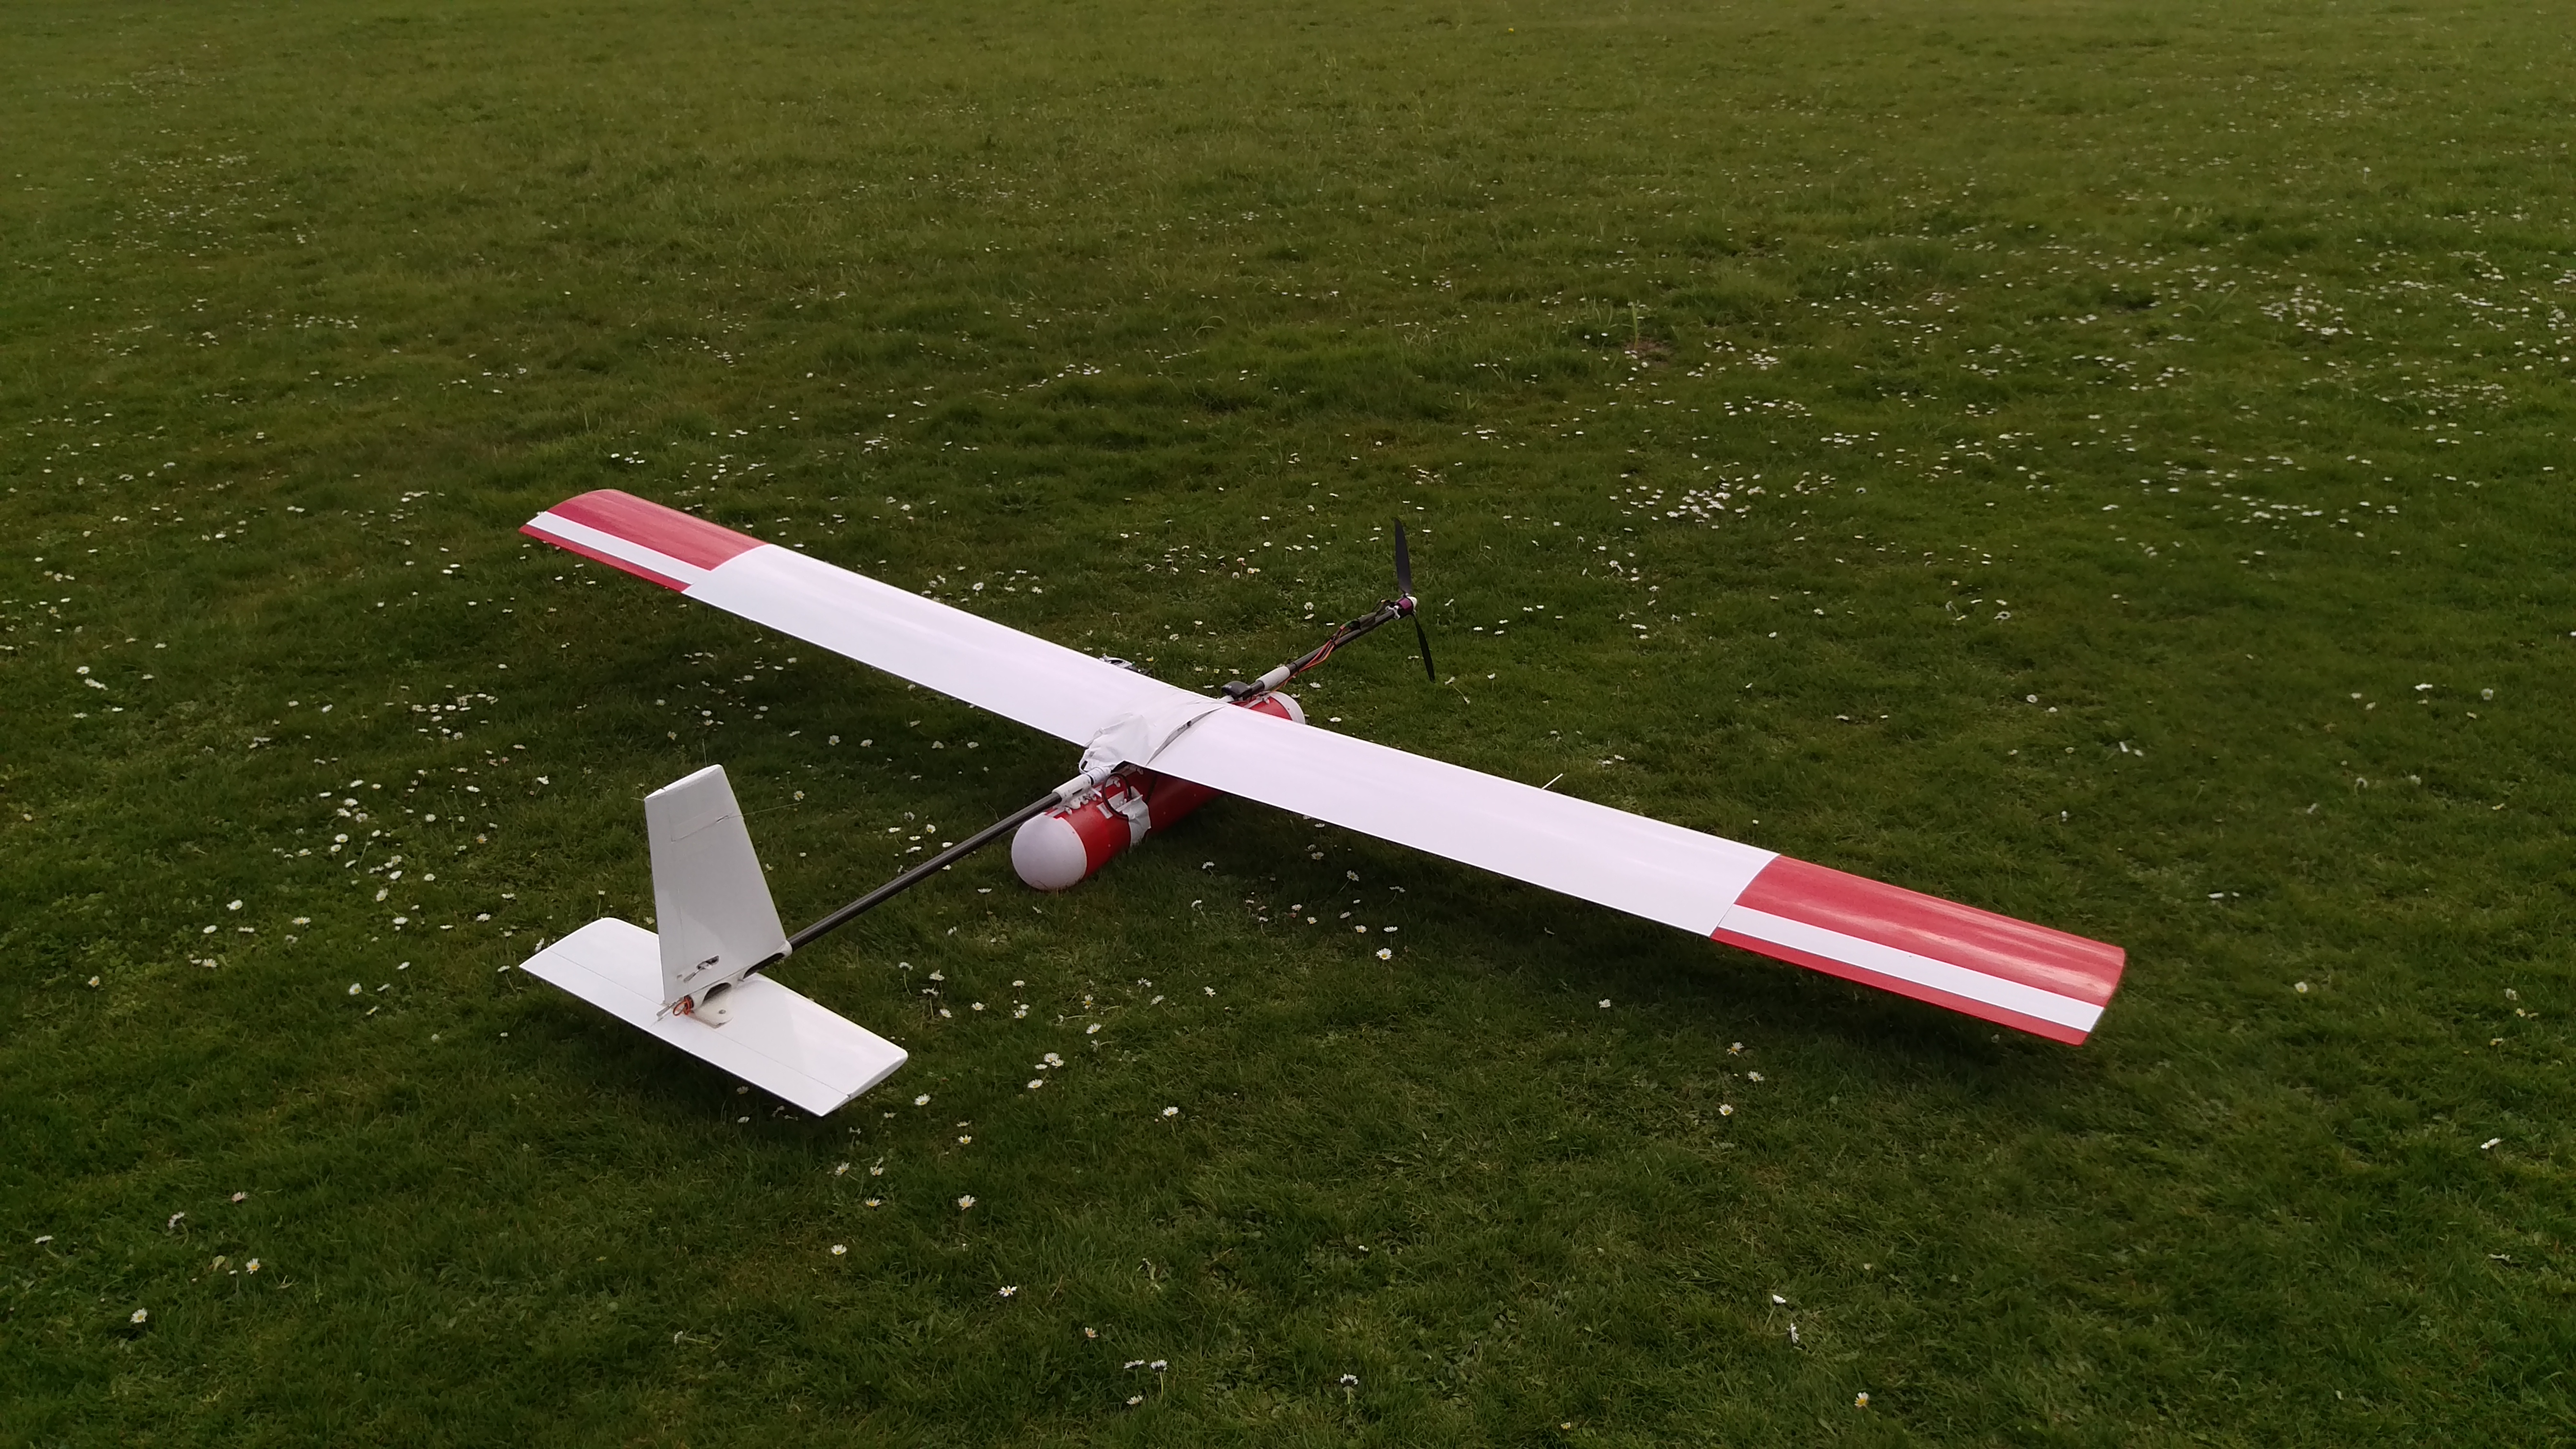
\includegraphics[width=0.9\textwidth]{bilder/Fotos/AUVSI_2015.jpg} 
\caption{Das AUVSI 2015 Modell im Einsatzzustand am Testflugplatz} 
\label{fig:Das AUVSI 2015 Modell in Einsatzzustand am Testflugplatz}
\end{figure}

Im Bild \ref{fig:Das AUVSI 2015 Modell in Einsatzzustand am Testflugplatz} ist der Gesamtaufbau des Flugzeugs zu sehen. Bisher sind der Einsatz von Rechteckigen Auftriebsflächen und Leitwerken sowie CFK-Rohren als Ausleger für Heck und Motorträger charakteristisch. Unter dem Zentralen Rumpfrohr ist der Zylinderförmige Nutzlastbehälter Montiert.


\clearpage


\section{Bisherige Flügelbauweise}

Die bisherigen Tragflügel sowie einige Leitwerksflächen wurden in der in Modellbaukreisen als \glqq Styro-Abachi\glqq{}  bekannt Bauweise ausgeführt. In diesem konkreten Fall werden die Tragflächen des AUVSI-UAV's ausgehend von einem Kern aus Polystyrol gefertigt. In einem ersten Schritt wird mit Hilfe einer 4-Achs CNC Heißdrahtschneidemaschine die gewählte Profilform (Clark-Y) aus einem Styroporkern geschnitten. In diesen Rohling werden anschließend Aussparungen für die Kabelschächte und die Servomotoren der Rudermaschinen eingebracht. Auf Ober- und Unterseite der Fläche wird Abachi Funier mit einer Schichtstärke von 0,6 mm verklebt. Dabei wird während der Aushärtephase des Klebstoffs ein Vakuumsack eingesetzt um die Festigkeit der Klebeverbindung zu steigern.
Auf beiden Ende werden Endrippen aus 3 mm starkem Ceibasperrholz aufgebracht. Die Kraftübertragung in die anschließenden Segmente wird durch, in die Polystyrolblöcke eingeklebte, CFK-Rohre realisiert. Daran anschließend erfolgt das Auskasten und Anschlagen der Ruderflächen.
Abschließend wird die Fläche mit heißklebender Kunststoffolie mit Hilfe eines Bügeleisens überzogen, um sie resistenter gegen Umwelteinflüsse zu machen.

Bei dieser Bauweise soll der Großteil der Zugspannungen vom aufgebrachen Abachi Funier in Faserrichtung aufgenommen werden. Der Polystyrolkern soll hingegen die Übertragung der Schubspannungen zwischen Ober- und Unterseite der Tragfläche gewährleisten und nimmt zusätzlich entstehenden Druck quer zur Oberfläche auf. Als problematischer Parameter, der die Biegefestigkeit der Gesamtstruktur erheblich reduziert, hat sich die Festigkeit der Klebeverbindung zwischen oberer Funierlage (Druck) und dem Polystyrolkern herauskristallisiert. Ein Versagen der Verklebung führt zum Abschälen des Funiers, was ein Druckbeulen der oberseitigen Funierlage nach sich zieht. Dadurch tritt ein Stabilitätsversagen ein.

Insgesamt hat sich diese Bauweise als sehr robust erwiesen und hat eine ausreichende Stabilität in allen Flugsituationen nachgewiesen.
Die Formabweichungen von der gewählten Profilform sind vergleichsweise gering. Dies setzt allerdings den Einsatz von korrekt gefertigten Werkzeugen während des Vakuumverfahrens vorraus. 

Nachteilig ist das vergleichsweise hohe Gewicht von 2,145\,$kg/m^2$ [AUVSI/Ecuador 2015].
Zusätzlich wird für die Fertigung ein einfacher Werkzeugbau benötigt und es müssen zahlreiche Arbeitsschritte, von denen manche überdurchnittliches handwerkliches Geschick erfordern, durchgeführt werden. Damit variiert die Qualität der Ergebnisse je nach Erfahrung und Sorgfalt des Personals deutlich. Gerade Fehler beim Vakuumverkleben der Funierschichten können das gesamte Tragflächensegment unbrauchbar machen. 

Bisher ist weder eine Vorauslegung noch eine Dimensionierung der Struktur für die erwarteten Lasten durchgeführt worden.

Erfahrungen aus Belastungs- und Überlastungsversuchen mit alten Tragflächen dieser Bauweise, lassen erwarten das die bisherige Struktur bedeutend zu stabil und schwer ist. 

\clearpage

\section{Verbesserungsziele}

Ziele dieser Arbeit und der durchgeführten Auslegung sollen Verbesserungen zur jetzigen Bauform in folgenden Bereichen sein:
\begin{itemize}
    \item Nachweis der Festigkeit der Fläche bei bekannten Sicherheiten und Lastgrenzen.
    \item Reduzierung des Flächengewichts durch bessere Ausnutzung der Materialkennwerte.
    \item Reduzierung des Anteils an anspruchsvoller Handarbeit und Steigerung des Anteils mechanisierter und werkzeugbasierter Fertigung.
    \item Einsatz einer möglichst profiltreuen Bauweise bis zu mindestens 25\% der Flächentiefe.
    \label{lst:Verbesserungsziele}
\end{itemize}


\section{Optimierungsgrenzen durch den Einsatz}

Die Optimierung des Flügels in Bauform und Materialwahl nach in \ref{lst:Verbesserungsziele} genannten Maßgaben ist durch eine Reihe von Situationen im Alltagseinsatz des Fluggeräts begrenzt, welche über den Statischen Flugzustand hinausgehen.

Das Fluggerät wird im Normalfall von einer kurzen Rampe mit einem Gummiseil im Flitschenstart gestartet. Dadurch entstehen kurzzeitig Lastvielfache von bis zu 3,5 g in X Richtung bis kurz über die Festgelegt Mindestfluggeschwindigkeit.
Auch ein Hochstart wurde für Einsätze in denen der Energieverbauch zum erreichen der Missionshöhe einen hohen Anteil hat an der Gesamtflugaufgabe hat disskutiert. 
Dadurch muss die Tragfläche kurzzeitig eine deutlich höhere Auftriebkraft ertragen als für den Statischen Reiseflug vorgesehen. 

Das Fluggerät unterliegt im Alltagseinsatz einer Reihe von Belastungen welche Atypisch zum regulären Flug sind. Beispielsweise werden die Flächen in Kisten Transportiert,sowie beim Auspacken und Montieren mit Handkraft auf Druck beansprucht. Die Fläche bedarf somit einer Ausreichenden Druckfestigkeit, oder aber einfache Methoden Beschädigungen durch unsachgemäßes Handling instandzusetzen.